% !TeX root = ../tesis.tex

\chapter{Técnica de integración finita}
\label{chapter:FIT}

\vspace*{7em}

La Técnica de Integración Finita (FIT), propuesta por primera vez por Weiland en 1976/1977 [1]. Este método numérico proporciona un esquema universal de discretización espacial. La Técnica de Integración Finita (FIT) reescribe las ecuaciones de Maxwell en su forma integral en una formulación discreta. El conjunto de ecuaciones algebraicas resultante, las Ecuaciones de Cuadrícula de Maxwell (MGE), son muy adecuadas para el análisis numérico.

\blindtext


\section{Celda dual}
\label{section:yee}

La Técnica de integración finita consiste en que a diferencia de FEM, las componentes del campo eléctrico y del campo magnético se definen en posiciones espaciales distintas dentro de cada celda \cite{yeeNumericalSolutionInitial1966}. En particular, las componentes del campo eléctrico se evalúan en los centros de las aristas de la celda, mientras que las componentes del campo magnético se definen en los centros de las caras. Esta disposición escalonada introduce de manera natural el concepto de malla dual. En este formalismo, el dominio computacional se discretiza mediante una malla primaria (primal grid), sobre la cual se definen ciertas magnitudes electromagnéticas, y una malla dual asociada, desplazada ortogonalmente respecto a la primera, donde se definen las magnitudes complementarias \cite{tafloveComputationalElectrodynamicsFinite2005}. En particular, los campos eléctricos se asocian típicamente a las aristas de la malla primaria, mientras que los campos magnéticos se asocian a las caras de la malla dual. Esta correspondencia refleja directamente la formulación integral de las ecuaciones de Maxwell, en la cual los campos se interpretan como cantidades promediadas sobre líneas, superficies o volúmenes.

Desde el punto de vista computacional, esta estructura de mallas duales se implementa explícitamente en herramientas como CST Microwave Studio®. Si bien el usuario visualiza principalmente la malla primaria en el entorno gráfico, internamente el solver construye una segunda malla dual, ortogonal a la primera. La discretización espacial de las ecuaciones de Maxwell se lleva a cabo simultáneamente sobre ambos sistemas de malla, lo que permite introducir los grados de libertad del problema en términos de cantidades integrales definidas sobre los elementos geométricos discretos.

Dentro de este marco de discretización basado en mallas duales, una cuestión central en la formulación de cualquier método numérico es la elección adecuada de las magnitudes desconocidas que se calcularán, es decir, las variables de estado del modelo. Dependiendo del enfoque adoptado, dichas variables pueden corresponder a potenciales vectoriales, potenciales escalares, potenciales de Hertz, componentes de los campos electromagnéticos o magnitudes derivadas de éstos. En el método de Integración Finita se adopta una formulación intrínsecamente integral, en la cual las variables de estado no son los campos puntuales, sino las denominadas tensiones y flujos de malla. Estas magnitudes escalares se definen como integrales de los campos eléctrico y magnético a lo largo de los elementos geométricos de las mallas primaria y dual, respectivamente. 
%
\begin{figure}[h!]
	\centering
	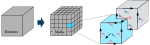
\includegraphics[width=14cm]{../../Figuras/FIT_grid.pdf}
	\caption{Contorno de integración $C$ conformado por cuatro curvas.}
	\label{fig:FIT_grid}
\end{figure}
%
